\documentclass[conference]{IEEEtran}
\usepackage{ifthen}
\usepackage{amssymb}
\usepackage{color}

\newboolean{showcomments}


\setboolean{showcomments}{true}

% useful to avoid size increasing for textbf command (in order to preserve alignment in tables)
\newsavebox\CBox
\def\textBF#1{\sbox\CBox{#1}\resizebox{\wd\CBox}{\ht\CBox}{\textbf{#1}}}

\ifthenelse{\boolean{showcomments}}
  {\newcommand{\nb}[2]{
    \fbox{\bfseries\sffamily\scriptsize\color{red}#1}
    {\sf\small$\blacktriangleright${\color{red}\textit{#2}}$\blacktriangleleft$}
   }
   \newcommand{\cvsversion}{\emph{\scriptsize$-$Id: macro.tex,v 1.9 2005/12/09 22:38:33 giulio Exp $}}
  }
  {\newcommand{\nb}[2]{}
   \newcommand{\cvsversion}{}
  }


\newcommand\RQ[1]{\textbf{RQ$_#1$}}
\newcommand\SIMONE[1]{\nb{SIMONE}{#1}}
\newcommand\GIO[1]{\nb{GIO}{#1}}
\newcommand\DARIO[1]{\nb{DARIO}{#1}}
\newcommand\ROCCO[1]{\nb{ROCCO}{#1}}
\newcommand\ANDREA[1]{\nb{ANDREA}{#1}}
\newcommand\FABIO[1]{\nb{FABIO}{#1}}
\newcommand\SEBA[1]{\nb{SEBA}{#1}}
\newcommand\ADELINA[1]{\nb{ADELINA}{#1}}

\newcommand\NEW[1]{\nb{NEW}{#1}}
\newcommand\TODO[1]{\nb{TODO}{#1}}
\newcommand\UPDATE[1]{\nb{TOUPDATE}{#1}}
\newcommand\CIT[1]{\nb{Cit.}{#1}}





\usepackage{cite}
\usepackage{comment}
\usepackage{enumerate}
\usepackage{graphicx, color}                       
\usepackage[usenames,dvipsnames]{xcolor}        
\usepackage[utf8]{inputenc}
\usepackage{amssymb,amsmath}\setlength{\parindent}{0in}
\usepackage{paralist}               
\usepackage{tabularx,ragged2e}                            
\usepackage{balance}                          
\usepackage{multirow}     
\usepackage{multicol}            
\usepackage{fancyvrb}       
\usepackage[TABBOTCAP]{subfigure}                         
\usepackage{tikz}
\usepackage{xspace}
\usepackage{amsmath}
\usepackage{hyperref}
\usepackage{bm}
\usepackage{epstopdf}
\usepackage{lipsum}
\usepackage{tcolorbox}
\usepackage{booktabs}
\usepackage{dblfloatfix}    % To enable figures at the bottom of page
  
\newcommand{\ie}{\emph{i.e.},\xspace}
\newcommand{\Ie}{\emph{I.e.},\xspace}
\newcommand{\eg}{\emph{e.g.},\xspace}
\newcommand{\Eg}{\emph{E.g.},\xspace}
\newcommand{\etal}{\emph{et al.}\xspace}

\newcommand\Giovanni[1]{\textbf{Giovanni}{#1}}
\newcommand\Adelina[1]{\textbf{Adelina}{#1}}
\newcommand\Fabio[1]{\textbf{Fabio}{#1}}
\newcommand\Sebastiano[1]{\textbf{Sebastiano}{#1}}
\newcommand\Lucas[1]{\textbf{Lucas}{#1}}

\newcommand{\sapienz}[0]{\textsc{Sapienz~}}
\newcommand{\monkey}[0]{\textsc{Monkey~}}
\newcommand{\tool}[0]{\textsc{ChangeAdvisor}}

\renewcommand{\arraystretch}{1.2}

\usepackage{listings}
\definecolor{mygreen}{rgb}{0,0.6,0}
\definecolor{mygray}{rgb}{0.5,0.5,0.5}
\definecolor{mymauve}{rgb}{0.58,0,0.82}
% === Per gli snippet =====================================
\lstset{
  backgroundcolor=\color{white},   % choose the background color; you must add \usepackage{color} or \usepackage{xcolor}
  basicstyle=\large,        		   % the size of the fonts that are used for the code
  breakatwhitespace=false,         % sets if automatic breaks should only happen at whitespace
  breaklines=true,                 % sets automatic line breaking
  captionpos=b,                    % sets the caption-position to bottom
  commentstyle=\color{mygreen},    % comment style
  deletekeywords={},			   % if you want to delete keywords from the given language
  escapeinside={\%*}{*)},          % if you want to add LaTeX within your code
  extendedchars=true,              % lets you use non-ASCII characters; for 8-bits encodings only, does not work with UTF-8
  frame=single,                    % adds a frame around the code
  keepspaces=true,                 % keeps spaces in text, useful for keeping indentation of code (possibly needs columns=flexible)
  keywordstyle=\color{blue},       % keyword style
%  language=Python,                 % the language of the code
  morekeywords={},            	   % if you want to add more keywords to the set
  numbers=none,                    % where to put the line-numbers; possible values are (none, left, right)
  numbersep=5pt,                   % how far the line-numbers are from the code
  numberstyle=\tiny\color{mygray}, % the style that is used for the line-numbers
  rulecolor=\color{black},         % if not set, the frame-color may be changed on line-breaks within not-black text (e.g. comments (green here))
  showspaces=false,                % show spaces everywhere adding particular underscores; it overrides 'showstringspaces'
  showstringspaces=false,          % underline spaces within strings only
  showtabs=false,                  % show tabs within strings adding particular underscores
  stepnumber=1,                    % the step between two line-numbers. If it's 1, each line will be numbered
  stringstyle=\color{mymauve},     % string literal style
  basicstyle=\scriptsize,
  tabsize=2,                       % sets default tabsize to 2 spaces
  title=\lstname,                  % show the filename of files included with \lstinputlisting; also try caption instead of title
  belowskip=1.0em,				   % sets the vertical space below	
  aboveskip=0.8em   		       % sets the vertical space above
}

\begin{document}

\title{ChangeAdvisor: A Change Requests Recommender Based on Android User Reviews}

%\author{\IEEEauthorblockN{Lucas Pelloni, Giovanni Grano,
%Adelina Ciurumelea \\ Sebastiano Panichella, Fabio Palomba and
%Harald C. Gall}
%\IEEEauthorblockA{University of Zurich,\\
%Department of Informatics, Switzerland\\
%lucas.pelloni@uzh.ch, \{grano,ciurumelea,panichella,palomba,gall\}@ifi.uzh.ch}}

\maketitle
\begin{abstract}
Android user reviews often contain precious information that can be profitably used to guide software maintenance activities. Nevertheless, because of their high frequency and lack of textual structure, analyzing the user feedback may result in a problematic and manual effort. In this paper, we describe ChangeAdvisor, a tool that (i) examines the structure, semantics, and sentiments of user reviews to distill change requests to be addressed; (ii) then, it leverages information retrieval approaches to localize the code artifacts that need to be changed. The quantitative and qualitative evaluation of ChangeAdvisor, involving 10 open source mobile apps and their original developers, showed a high accuracy of the presented tool in (i) distilling and clustering user change requests and (ii) linking the source code components that need to be changed to accomodate such requests. In evaluating ChangeAdvisor we found that the original developers of the analyzed apps confirm the practical usefulness of the provided software change recommendations.
\end{abstract}

\begin{IEEEkeywords}
\footnotesize
Mobile Applications, User Reviews Analysis
\end{IEEEkeywords}

% Introduction
\section{Introduction}
\label{sec:intro}
%User feedback plays a paramount role in the development and maintenance of mobile applications. 
In order to hit the market as quick as possible and to win market share, the software development industry has embraced a paradigm of short and iterative development cycles. Especially in the world of mobile applications, where the advent of mobile app stores has made it easier than ever to manage updates. With the app stores, came also the possibility of users to voice their opinion regarding software in the form of short texts and numerical scores. These reviews are free text and may contain information relevant for developers~\cite{inukollu2014factors}, albeit informally and unstructured. The information contained ranges from problem reports~\cite{Pagano:2013:RE}, to feedback regarding features~\cite{Guzman:2014:RE}, requests for enhancements~\cite{iacob2013retrieving} and new features~\cite{Pagano:2013:RE,galvis2013analysis}, and comparisons with competing apps.
Thus app stores provide provide people a way to give their opinion in a quick and simple manner, but it is also a powerful crowd feedback mechanism, which enables developers to discover and fix potential bugs as soon as possible, as well as redirecting the project direction to fulfill market requirements.

Thus, as a natural consequence, research started to come up with ways to capitalize on this wealth of information. Harman \textit{et al.}~\cite{Harman:MSR:2012} introduced the concept of \textit{App Store Mining} as a form of \textit{Mining Software Repositories}.

There are difficulties in exploiting this information, however. The various app stores, usually provide only limited support for sorting and aggregating this data to derive requirements~\cite{abelein2013does}. Considering the sheer amount of reviews popular apps receive, it is sometimes not feasible at all to read them all, even less to distinguish which ones are relevant for maintenance tasks.

Thus researchers practitioners have come up with new approaches to distinguish relevant reviews~\cite{iacob2013retrieving,panichella2015can,oh2013facilitating}. Many of these approaches however only classify reviews, without considering semantics. Additionally there exists no way of correlating user feedback to the actual code components that need to be changed. 

% Design
\section{\tool{}} 
%\section{Approach}
\label{sec:design}
This section briefly describes the approach and technologies we employed. 
\tool{} is a tool built with a set of different technologies: the core part, the back-end, is written in Java while the front-end application is written in React.
This section reports the main characteristics of \tool{}, as well as details about its architecture and inner-working.

\subsection{Approach Overview}
The \tool{} approach was first introduced by Palomba \textit{et. al}~\cite{Palomba2017}. The goal is to extract feedback relevant to software maintenance tasks from user reviews and suggest locations in code where improvements should be made. 
It consists of 4 main steps:
\begin{itemize}
\item user feedback classification (i.e. bug fixing, feature requests and enhancements);
\item source code and user feedback preprocessing;
\item user feedback clustering to create groups of reviews discussing the same changes;
\item determining code elements related to the reviews clusters.
\end{itemize}

%
% DESIGN GOALS
%
\subsection{Design Goals}
%\tool{} is designed with the main goal to link user feedback, discussing changes in a high-level language, such as feature requests and bug reports, to the source code components that will require modification in order to fulfill said change requests.
The newest iteration of \tool{} was devised to improve performance and usability. In order to support this goal, \tool{} leverages a database to cache computation results and improve search performance. It includes a user-interface in the form of a web application, which developers can use to easily import user reviews and source code. For reasons of space, screenshots of the user interface can be found on the tool's web page.
In addition, it is also possible to update \tool{}'s configuration, start jobs manually, and view a dashboard which includes information such as a timeseries of number of reviews vs. average of reviews, distribution of reviews based on category and labels representing the various review clusters.

Tools to import source code and user feedback are provided. Source code can be imported from repositories (at the moment only git is supported, but others will be added at a later date). Review data can be imported in two ways: (i) via a review miner; (ii) from the file system. All import tools can be configured and started through the UI.

%
% ARCHITECTURE
%
\begin{figure*}[!h]
    \centering
    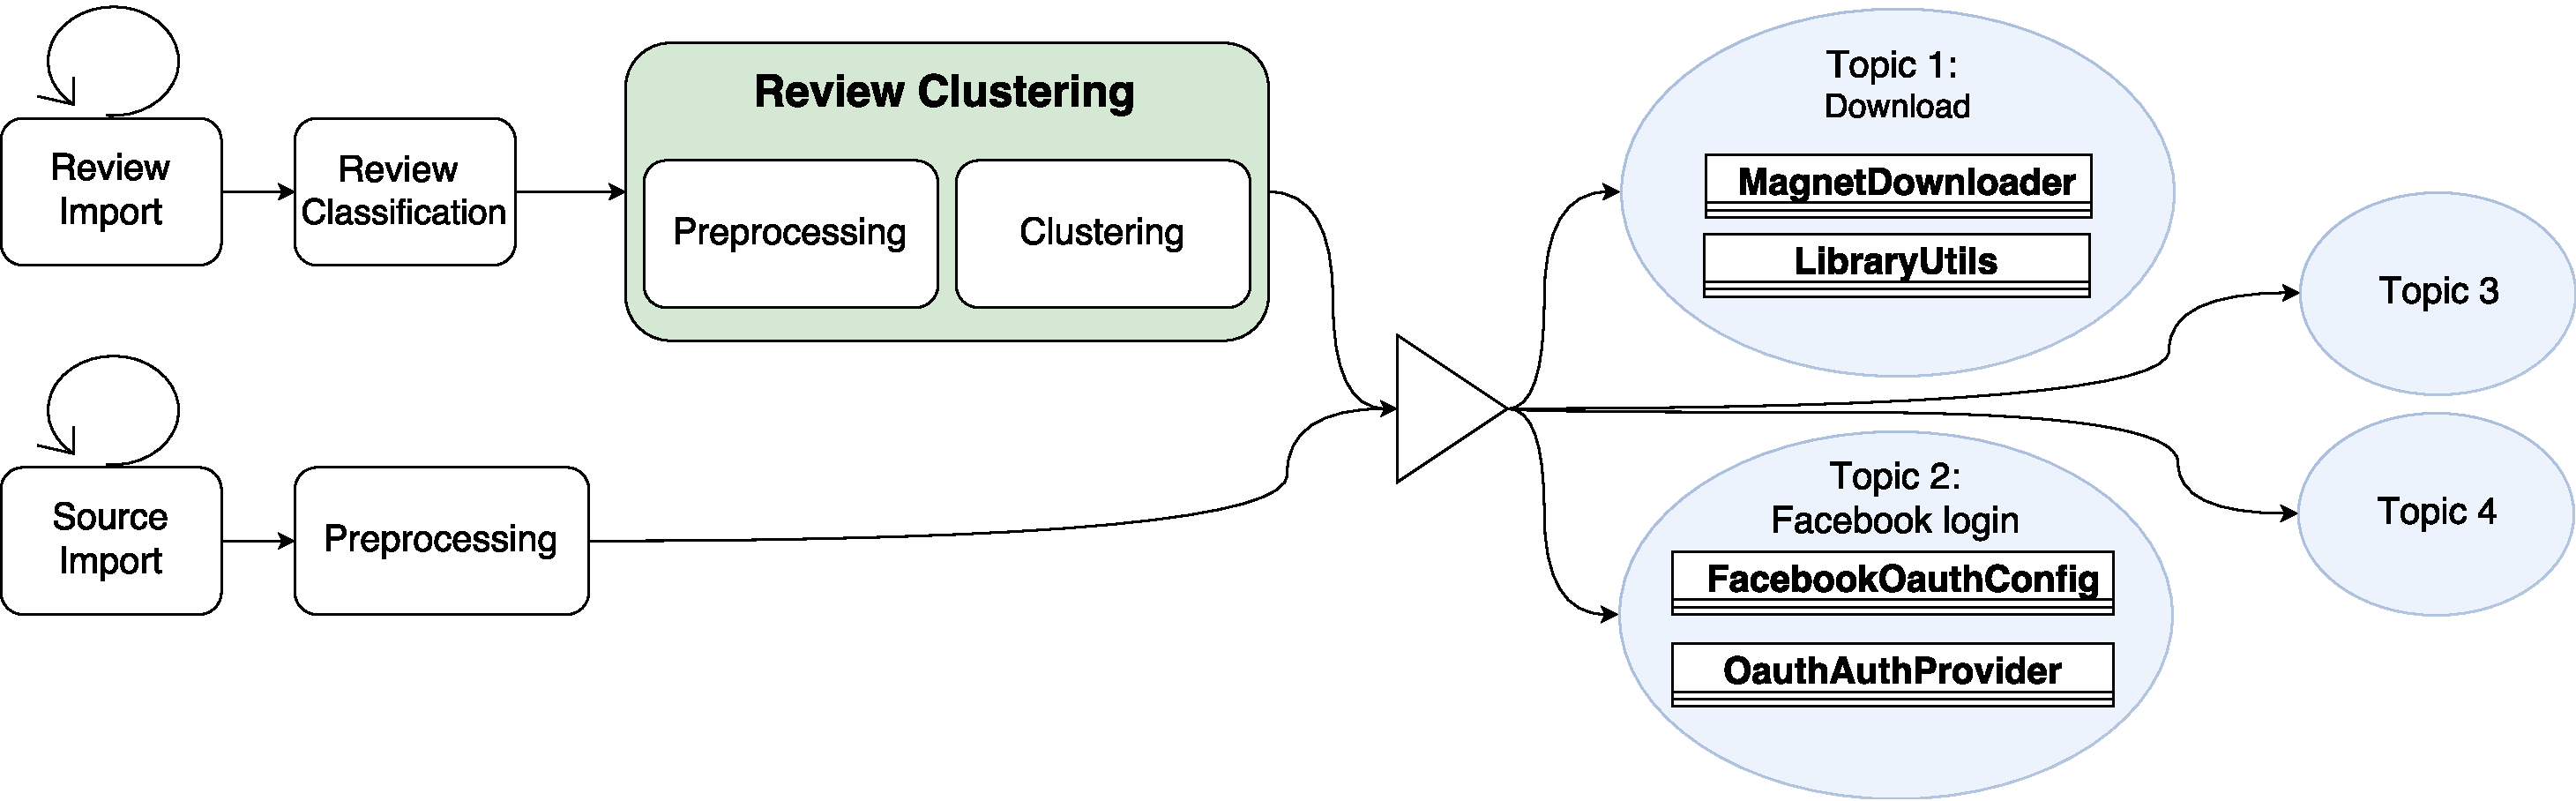
\includegraphics[scale=0.3]{imgs/ChangeAdvisorPipeline.pdf}
    \caption{Change Advisor Processing Pipeline}
    	\label{fig:architecture}
\end{figure*}

\subsection{\tool{} Architecture}
The overall architecture of \tool{} is depicted in Figure \ref{fig:architecture}.
As mentioned previously, the tool is divided in a client-side application and a back-end.

The back-end represents the core of \tool{}. The entirety of the logic is implemented at this level. On a logical level, this system can be divided in three components: (i) the \textit{Review Pipeline} that handles the import and preprocessing of user feedback; (ii) the \textit{Source Code Pipeline} which imports source code and preprocessing of source code components; (iii) the \textit{Linking}, which represents the core feature of the \tool{} approach, i.e. the link between the source code component and the user feedback referring such elements.



The back-end was written in Java upon Spring Boot and fully leverages the Spring Framework: Spring REST for the HTTP API; Spring Data for database access; Spring Batch for long running jobs. 
The front-end was written in React and communicates with the back-end via the aforementioned API.
Given that most processes of \tool{} are long running, we leverage the database to persist the results of the various steps of the tool in order to never have to recompute previous results. Additionally, we leverage the database for costly search and aggregation operations.

%The back-end represents the core of \tool{}. The entirety of the logic is implemented at this level. On a logical level, this system can be divided in three components: (i) the \textit{Review Pipeline} that handles the import and preprocessing of user feedback; (ii) the \textit{Source Code Pipeline} which imports source code and preprocessing of source code components; (iii) the \textit{Linking}, which represents the core feature of the \tool{} approach, i.e. the link between the source code component and the user feedback refering such elements.

The upcoming sections will further detail both front- as well as back-end and their composing components.

%
% The Review SUBSYSTEM
%
\subsection{The Review Subsystem}

%The aim of this subsystem is to facilitate the fetching and processing of user feedback into clusters that can then be used as input for the linking algorithm.

This system can logically be seen as a sequence of four steps: (i) review import which can be configured based on a schedule to automatically mine user reviews; (ii) the review classification step where we automatically classify reviews using a feedback classifier, into labeled categories representing whether a review represents a feature request (\texttt{FEATURE REQUEST}) or a bug request (\texttt{BUG REQUEST)}; (iii) the review preprocessing step in order to clean the user feedback from textual noise which might hinder the accuracy of the clustering and linking~\cite{Palomba2017}; (iv) the clustering step which groups together user reviews discussing the same change request.

\paragraph{Review import} 
\tool{} relies for the first step on an external tool, a Java-built scraper tool~\cite{Grano:2017} that relies on PhantomJS\footnote{\url{http://phantomjs.org}} and Selenium\footnote{\url{http://www.seleniumhq.org}} to navigate to and extract the reviews from the Google Play Store.

\paragraph{Review classification}
Once the reviews are mined, we employ another external tool, a review classifier~\cite{panichella2016ardoc} which uses Natural Language Processing (NLP), Sentiment and Text Analysis (SA \& TA)~\cite{panichella2016ardoc} in order to process the reviews into categories such as \textit{FEATURE REQUEST} and \textit{BUG REPORT}. We do this to discern the ones that are useful for linking later on.

\paragraph{Preprocessing}
Since user feedback tends to be rather informal and noisy~\cite{Mernik:2005}, we first processes them into a suitable format for textual analysis. Thus, to prepare the reviews for clustering, we apply the following NLP noise removal steps: contraction expansion, stopword removal, and stemming~\cite{Palomba2017}. We then remove all documents which are too short, to clearly convey a change request. This results in a collection of bag of words which can then be used as input to a clustering algorithm.

\paragraph{Clustering}
The goal of this step is to build clusters of reviews discussing the same change requests. Consider the following example of two reviews discussing the same problem, taken verbatim from the reviews of \textit{AnkiDroid Flashcards}~\footnote{AnkiDroid Flashcards: \url{https://play.google.com/store/apps/details?id=com.ichi2.anki&hl=en}}: \begin{enumerate}
\item  Crashing constantly It's crashing when I try to take a photograph for a flash card, has been for weeks, going to uninstall it. […]
\item Hi guys. The app is great, but when i want to add image to the answer through cammera it crashes. […]
\end{enumerate}
Ideally, at the end of this step we have groups of reviews semantically similar to each other. These clusters will then be fed to the linking algorithm, as one of the inputs. We use clustering for two reasons: (i) as has been shown in the work of Palomba \textit{et al.}~\cite{Palomba2017} linking single reviews tends to return poor results, and (ii) clustering allows us to group together feedback referring ideally to the same, or at the very least, similar change request, thus avoiding duplicates and making the system more comprehensible and generally easier to follow for the developer. \tool{} performs two separate approaches to clustering. As with the original \tool{} paper~\cite{Palomba2017} we use Hierarchical Dirichlet Process (HDP), proposed by Teh \textit{et al.}~\cite{teh2005sharing}. HDP is an extension of the LDA algorithm where the number of topics is not known a priori. The \texttt{HierarchicalDirichletProcess} class implementing this approach, is a Java port of the \texttt{hdpla} python script that was used in the \tool{} paper~\cite{Palomba2017}.
Additionally, we attempt to create clusters by computing the \textit{Term-frequency inverse-document-frequency} (tf-idf) score over the N-grams of all reviews, and then picking the N-grams with the highest score and fetching all reviews containing said N-gram. 

Regardless of the clustering technique employed, at the end, we will have a set of processed reviews that we can use for linking. The return types of both clustering algorithms implement the \texttt{LinkableReview} interface, allowing the linker to use any of the two. Finally, both outputs are persisted to the database. By doing this, we do not need to compute new clusters each time we want to run the \textit{linker}. The clusters are only recomputed when new reviews are imported into \tool{}.

%
% Source code SUBSYSTEM
%
\subsection{The Source Code Subsystem}

The goal of this subsystem is to provide an easy to use interface to automatically import and process source code into a format that \tool{} can use as input to its linking algorithm. 
\paragraph{Source code import} 
Via the web interface a user can easily enter the url of the git repository. \tool{} will then automatically clone the repository, parse the code and divide it in its elements. We define a \textit{source code element} as the basic building blocks of an application, i.e. a \textit{class} in Java. We only keep classes (normal, nested and static nested) and enums. We discard interfaces as they do not implement any logic and would thus rarely be targets for change requests. To do so we use the JavaParser library \footnote{\url{http://javaparser.org}}. This library creates an Abstract Syntax Tree (AST) which can then be traversed using the visitor pattern. Thus, we traverse the tree and read the public API and comments of each class, creating a \textit{source code element}.

\paragraph{Source code preprocessing}
After parsing, we process each code element as we did with the review pipeline~\cite{Palomba2017,BaezaYates:1999}.
We split composed identifiers, such as camelCase and snake\_case, we remove special characters, english and programming stop words and stem each token using Porter's stemmer~\cite{porter1980algorithm}. from each code element to produce bag of tokens which we then persist in the database, ready to be used for the linking algorithm. 

%
% LINKING
%
\subsection{Linking}
The linking between the source code elements and the user reviews represents the core of \tool{}. After the previous steps of the two pipelines, we the preprocessed reviews and source code elements are retrieved from the database.
Each two bag of words (one of each type) are compared using the Dice similarity coefficient \cite{dice1945measures}, defined as follow:
\begin{equation*}
	\operatorname{Dice}\left(\mathit{cluster}_{i}, \mathit{source}_{j}\right) = \frac{\left|\mathit{W}_{\mathit{cluster}_{i}} \cap \mathit{W}_{\mathit{source}_{j}}\right|}{\min\left(\left|\mathit{W}_{\mathit{cluster}_{i}}\right|, \left|\mathit{W}_{\mathit{souce}_{j}}\right|\right)}
\end{equation*}
where $\mathit{W}_{\mathit{cluster}_{i}}$represents the set of words contained in cluster $i$. $\mathit{W}_{\mathit{source}_{j}}$ represents the set of words contained in the source code element $j$.
We normalize with respect to the shortest document, because user feedback is, in most cases, considerably shorter than our source code elements. Due to the normalization step, the Dice coefficient range is [0, 1].
The tool, then, links source code and reviews having a Dice score higher than 0.5 (in a range between $\left[0, 1\right]$). When linking, we keep a reference to the original (non-preprocessed) reviews. This is done in order to present the end-user with the context of the original feedback.


% Evaluation
\section{Evaluation}
\label{sec:evaluation}
\input{evaluation}


% Demo Remarks
\section{Demo Remarks}
\label{sec:remarks}
\input{conclusions}

%\newpage
%\balance
\bibliographystyle{abbrv}
\bibliography{biblio}  

\end{document}
